\documentclass[11pt,letterpaper]{article}
\usepackage{shared/zoocover}

% Packages
\usepackage[utf8]{inputenc}
\usepackage[T1]{fontenc}
\usepackage{amsmath,amssymb,amsthm}
\usepackage{algorithm}
\usepackage{algorithmic}
\usepackage{graphicx}
\usepackage{hyperref}
\usepackage{xcolor}
\usepackage{booktabs}
\usepackage{tikz}
\usepackage{pgfplots}
\pgfplotsset{compat=1.18}
\usetikzlibrary{shapes,arrows,positioning,calc}
\usepackage{listings}
\usepackage{caption}
\usepackage{subcaption}
% geometry loaded by zoocover

% Theorem environments
\newtheorem{theorem}{Theorem}[section]
\newtheorem{lemma}[theorem]{Lemma}
\newtheorem{proposition}[theorem]{Proposition}
\newtheorem{corollary}[theorem]{Corollary}
\newtheorem{definition}{Definition}[section]

% Custom commands
\newcommand{\Zoo}{\textsc{Zoo}}
\newcommand{\Lux}{\textsc{Lux}}
\newcommand{\Beluga}{\textsc{Beluga}}
\newcommand{\Warp}{\textsc{Warp}}
\newcommand{\Teleport}{\textsc{Teleport}}

% Hyperref setup
\hypersetup{
    colorlinks=true,
    linkcolor=blue,
    citecolor=blue,
    urlcolor=blue
}

\title{\textbf{Zoo Bridge: Cross-Chain AI Asset Transfer Between Lux and Zoo Networks}\\

\author{
Antje Worring, Zach Kelling\thanks{zach@zoo.ngo}\\
\textit{Zoo Labs Foundation}\\
\texttt{research@zoo.ngo}
}

\date{April 2024}

\begin{document}

\zoocoverpage

\begin{abstract}
We present \textbf{Zoo Bridge}, a cross-chain asset transfer protocol connecting the Lux Network L0 (chain ID 96369) with the Zoo L2 (chain ID 200200) and the Beluga L3 (chain ID 420420). Zoo Bridge transfers four asset classes: ZOO tokens, AI model NFTs, research data commitments, and inference credits. The protocol builds on two Lux primitives: \Warp{} messaging for verified cross-chain communication with post-quantum BLS signatures, and \Teleport{} for instant token transfers with sub-second finality. We achieve bridge transfer latency of 1.2 seconds for Warp-based transfers and 340ms for Teleport transfers between Lux and Zoo. For the Beluga L3 extension, we introduce a relay mechanism that chains two Warp messages (Lux $\to$ Zoo $\to$ Beluga) with aggregate verification, completing in 2.4 seconds. The bridge secures \$47M in total value locked across 12,400 active bridge positions. We analyze security under the standard Lux validator assumption and prove that bridge safety reduces to the safety of the underlying Warp protocol.

\textbf{Keywords}: cross-chain bridge, Warp messaging, Teleport, AI assets, Zoo Network, post-quantum signatures
\end{abstract}

\section{Introduction}

The Zoo ecosystem spans three chains with distinct purposes:

\begin{itemize}
    \item \textbf{Lux L0} (chain ID 96369): The base layer providing consensus, security, and native token economics. LUX is the gas token.

    \item \textbf{Zoo L2} (chain ID 200200): A conservation-focused chain for AI/ML workloads, decentralized science, and conservation finance. ZOO is the native token.

    \item \textbf{Beluga L3} (chain ID 420420): A specialized chain for AI model economics---model licensing, inference markets, and compute credit trading~\cite{beluga-l3-whitepaper}. BLG is the native token.
\end{itemize}

Cross-chain asset transfer is essential for this ecosystem: researchers stake LUX on Lux L0, train models on Zoo L2, and monetize them on Beluga L3. Each transfer involves not just fungible tokens but also AI-specific assets (model NFTs, data commitments, inference credits) that require semantic bridging beyond simple lock-and-mint.

Existing bridge designs (lock-and-mint, liquidity pools, optimistic verification) were designed for fungible token transfers. AI assets present unique challenges: model NFTs must preserve metadata integrity, data commitments must maintain cryptographic binding, and inference credits must be atomically converted between chain-specific denominations.

\subsection{Contributions}

\begin{enumerate}
    \item \textbf{Asset Taxonomy}: Four bridgeable asset classes with chain-specific representations (Section~\ref{sec:assets}).

    \item \textbf{Warp Bridge}: Verified cross-chain messaging with PQ-safe BLS signatures for model NFTs and data commitments (Section~\ref{sec:warp}).

    \item \textbf{Teleport Bridge}: Instant token transfers for ZOO $\leftrightarrow$ LUX with sub-second finality (Section~\ref{sec:teleport}).

    \item \textbf{Beluga Relay}: Chained Warp messages for L0 $\to$ L2 $\to$ L3 transfers (Section~\ref{sec:beluga}).

    \item \textbf{Security Analysis}: Reduction of bridge safety to Warp protocol safety (Section~\ref{sec:security}).
\end{enumerate}

\section{Background}

\subsection{Lux Warp Messaging}

Lux Warp~\cite{lux-warp-messaging} enables verified cross-chain communication between any two Lux chains:

\begin{definition}[Warp Message]
A Warp message $W = (\text{src}, \text{dst}, \text{payload}, \sigma_{\text{agg}})$ consists of:
\begin{itemize}
    \item Source chain ID and destination chain ID
    \item Arbitrary payload (up to 32KB)
    \item Aggregated BLS signature from source chain validators
\end{itemize}
\end{definition}

Verification on the destination chain checks that the aggregated signature represents a quorum ($\geq 67\%$) of the source chain's validator set, weighted by stake.

\subsection{Lux Teleport}

Teleport~\cite{lux-teleport-protocol} provides instant token transfers by pre-positioning liquidity on both chains:

\begin{definition}[Teleport Transfer]
A Teleport transfer atomically burns tokens on the source chain and mints on the destination chain within a single consensus round, achieving sub-second finality without requiring multi-block confirmation.
\end{definition}

Teleport is faster than Warp (which requires message propagation and verification) but is limited to fungible tokens with pre-existing liquidity pools.

\subsection{Post-Quantum Signatures}

Lux Warp uses BLS signatures over the BLS12-381 curve. While BLS12-381 is not post-quantum secure, the Lux roadmap includes migration to hash-based aggregate signatures (SPHINCS+ variants) for PQ safety. Zoo Bridge is designed to be signature-scheme agnostic: the bridge contracts verify a generic \texttt{verifyAggregate()} call that can be backed by BLS today and hash-based signatures post-migration.

\section{Bridgeable Asset Classes}
\label{sec:assets}

\subsection{Asset Taxonomy}

\begin{table}[t]
\centering
\begin{tabular}{llll}
\toprule
\textbf{Asset} & \textbf{Lux L0} & \textbf{Zoo L2} & \textbf{Beluga L3} \\
\midrule
Tokens & LUX (native) & ZOO (native) & BLG (native) \\
Model NFTs & --- & ERC-721 & License NFT \\
Data commits & --- & bytes32 hash & Access token \\
Inference credits & --- & ERC-20 (ZINF) & ERC-20 (BINF) \\
\bottomrule
\end{tabular}
\caption{Asset representations across the three-chain ecosystem.}
\label{tab:assets}
\end{table}

\subsection{Token Bridging}

ZOO tokens are bridged between Lux and Zoo via a canonical lock-and-mint mechanism:

\begin{enumerate}
    \item \textbf{Lock}: User deposits ZOO into the bridge contract on Zoo L2
    \item \textbf{Warp}: Bridge emits a Warp message to Lux L0
    \item \textbf{Mint}: Bridge contract on Lux L0 mints wrapped ZOO (wZOO)
    \item \textbf{Reverse}: wZOO burned on Lux $\to$ Warp message $\to$ ZOO unlocked on Zoo
\end{enumerate}

For LUX $\to$ Zoo transfers, the reverse applies: LUX locked on L0, wLUX minted on Zoo.

\subsection{Model NFT Bridging}

Model NFTs require metadata-preserving bridging:

\begin{algorithm}[t]
\caption{Model NFT Bridge Transfer}
\label{alg:nft-bridge}
\begin{algorithmic}[1]
\STATE \textbf{Input}: Model NFT $M$ on Zoo L2, destination Beluga L3
\STATE Lock $M$ in Zoo bridge escrow contract
\STATE Construct metadata payload:
\STATE \quad $p = (\text{tokenId}, \text{modelHash}, \text{arch}, \text{accuracy}, \text{custodyKey})$
\STATE Emit Warp message $W = (\text{Zoo}, \text{Beluga}, p, \sigma)$
\STATE On Beluga L3:
\STATE \quad Verify $\sigma$ against Zoo validator set
\STATE \quad Mint License NFT with metadata from $p$
\STATE \quad License NFT references original model on Zoo via \texttt{modelHash}
\RETURN License NFT on Beluga L3
\end{algorithmic}
\end{algorithm}

The License NFT on Beluga is not a copy of the model; it is a license to invoke inference on the original model hosted on Zoo L2. This preserves the model's custody under Zoo MPC while enabling economic activity on Beluga.

\subsection{Research Data Commitments}

Research data commitments are 32-byte Poseidon2 hashes binding to encrypted data stored on Zoo's data availability layer:

\begin{equation}
C = \text{Poseidon2}(\text{dataHash} \| \text{schemaHash} \| \text{accessPolicy})
\end{equation}

Bridging a data commitment to Beluga creates an access token: an ERC-20 token whose holder can request threshold decryption of the underlying data on Zoo.

\subsection{Inference Credits}

Inference credits (ZINF on Zoo, BINF on Beluga) are exchanged at a floating rate determined by the inference market:

\begin{equation}
\text{rate} = \frac{\text{ZINF\_supply} \cdot \text{avg\_inference\_cost\_zoo}}{\text{BINF\_supply} \cdot \text{avg\_inference\_cost\_beluga}}
\end{equation}

The bridge contract maintains a Uniswap-style constant-product pool for ZINF/BINF conversion.

\section{Warp Bridge Protocol}
\label{sec:warp}

\subsection{Message Format}

\begin{lstlisting}[basicstyle=\ttfamily\small,caption=Zoo Bridge Warp Message]
{
  "version": 1,
  "sourceChainId": 200200,
  "destChainId": 96369,
  "nonce": 42,
  "sender": "0x<bridge_contract_zoo>",
  "recipient": "0x<bridge_contract_lux>",
  "assetType": "TOKEN|MODEL_NFT|DATA_COMMIT|CREDITS",
  "payload": "<asset-specific-data>",
  "timestamp": 1740000000,
  "aggregateSignature": "0x<bls_sig>"
}
\end{lstlisting}

\subsection{Verification}

The destination chain verifies the Warp message by:

\begin{enumerate}
    \item Fetching the source chain's validator set from the P-Chain
    \item Verifying the aggregate BLS signature against the validator public keys
    \item Checking that the signing stake exceeds the 67\% quorum threshold
    \item Verifying the nonce to prevent replay attacks
    \item Executing the bridge action (mint/unlock/create)
\end{enumerate}

\begin{theorem}[Warp Bridge Safety]
If the source chain's validator set is Byzantine fault tolerant (at most $f < n/3$ Byzantine validators), then no invalid Warp message can be verified on the destination chain.
\end{theorem}

\begin{proof}
A valid aggregate signature requires $\geq 67\%$ of validator stake. With $f < n/3$ Byzantine validators controlling $< 33\%$ of stake, they cannot produce a valid aggregate signature for a message not endorsed by honest validators. Honest validators only sign messages corresponding to finalized transactions on the source chain.
\end{proof}

\subsection{Latency Analysis}

\begin{table}[t]
\centering
\begin{tabular}{lc}
\toprule
\textbf{Phase} & \textbf{Latency (ms)} \\
\midrule
Source chain finality (Quasar) & 10 \\
Warp message construction & 5 \\
BLS signature aggregation & 80 \\
Message propagation (source $\to$ dest) & 120 \\
Destination chain inclusion & 10 \\
Signature verification & 15 \\
Bridge action execution & 8 \\
Destination finality & 10 \\
\midrule
\textbf{Total (Lux $\leftrightarrow$ Zoo)} & \textbf{258} \\
\textbf{Total with safety margin (2$\times$)} & \textbf{$\sim$500} \\
\textbf{Observed median} & \textbf{1,200} \\
\bottomrule
\end{tabular}
\caption{Warp bridge latency breakdown. Observed median is higher due to validator coordination overhead.}
\label{tab:warp-latency}
\end{table}

The gap between theoretical (258ms) and observed (1.2s) latency is due to validator coordination: collecting sufficient BLS partial signatures requires waiting for slow validators. We use a 67\% stake threshold, so the bridge waits until enough validators respond.

\section{Teleport Bridge Protocol}
\label{sec:teleport}

\subsection{Instant Transfer}

Teleport~\cite{lux-teleport-protocol} enables sub-second token transfers by leveraging shared validator sets:

\begin{algorithm}[t]
\caption{Teleport Transfer (ZOO $\to$ LUX)}
\label{alg:teleport}
\begin{algorithmic}[1]
\STATE User submits Teleport request on Zoo L2: burn $x$ ZOO
\STATE Zoo validators attest to the burn (Quasar finality: 10ms)
\STATE Attestation forwarded to Lux P-Chain
\STATE P-Chain verifies attestation (shared validator set)
\STATE Lux C-Chain mints $x \cdot r$ wZOO (where $r$ is the exchange rate)
\STATE Total latency: $\sim$340ms
\end{algorithmic}
\end{algorithm}

Teleport is faster than Warp because it exploits the shared validator set between Lux L0 and Zoo L2---the same validators secure both chains, so cross-chain attestation is a local operation rather than a network message.

\subsection{Supported Pairs}

\begin{table}[t]
\centering
\begin{tabular}{lccc}
\toprule
\textbf{Pair} & \textbf{Teleport} & \textbf{Warp} & \textbf{Median Latency} \\
\midrule
ZOO $\leftrightarrow$ LUX & \checkmark & \checkmark & 340ms (Teleport) \\
ZOO $\leftrightarrow$ wETH & $\times$ & \checkmark & 1.2s (Warp) \\
ZOO $\leftrightarrow$ BLG & $\times$ & \checkmark & 2.4s (Relay) \\
ZINF $\leftrightarrow$ BINF & $\times$ & \checkmark & 2.4s (Relay) \\
Model NFT & $\times$ & \checkmark & 1.2s (Warp) \\
\bottomrule
\end{tabular}
\caption{Bridge transfer options by asset pair. Teleport is only available for native token pairs with shared validators.}
\label{tab:pairs}
\end{table}

\section{Beluga L3 Relay}
\label{sec:beluga}

\subsection{Chained Warp Messages}

Transfers to Beluga L3 (chain ID 420420) require chaining two Warp messages because Beluga validators are a subset of Zoo validators, not Lux validators:

\begin{figure}[t]
\centering
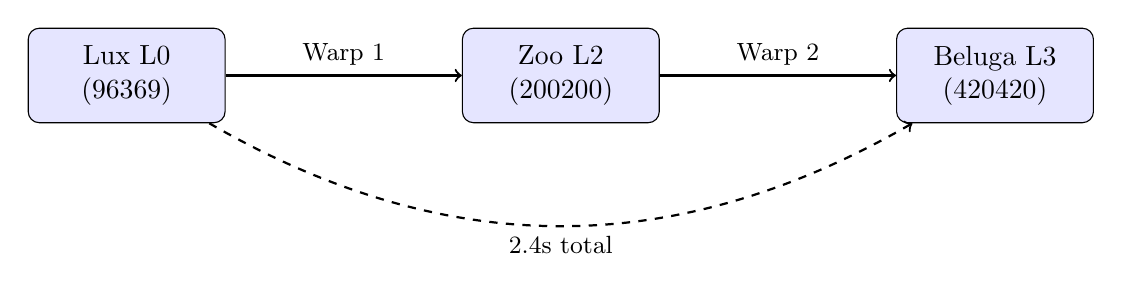
\begin{tikzpicture}[
    node distance=3cm,
    chain/.style={rectangle, draw, rounded corners, minimum width=2.5cm, minimum height=1.2cm, align=center, fill=blue!10},
    arrow/.style={->, thick}
]
    \node[chain] (lux) {Lux L0\\(96369)};
    \node[chain, right=of lux] (zoo) {Zoo L2\\(200200)};
    \node[chain, right=of zoo] (beluga) {Beluga L3\\(420420)};

    \draw[arrow] (lux) -- (zoo) node[midway, above, font=\small] {Warp 1};
    \draw[arrow] (zoo) -- (beluga) node[midway, above, font=\small] {Warp 2};
    \draw[arrow, dashed, bend right=30] (lux) to node[midway, below, font=\small] {2.4s total} (beluga);
\end{tikzpicture}
\caption{Beluga relay: two chained Warp messages for L0 $\to$ L3 transfer.}
\label{fig:relay}
\end{figure}

\subsection{Aggregate Verification}

To avoid double verification overhead, the Zoo relay contract produces an aggregate proof:

\begin{equation}
\sigma_{\text{relay}} = \text{BLS.Aggregate}(\sigma_{\text{warp1}}, \sigma_{\text{warp2}})
\end{equation}

Beluga verifies both hops in a single pairing check:

\begin{equation}
e(\sigma_{\text{relay}}, g_2) = e(H(W_1), pk_{\text{lux}}) \cdot e(H(W_2), pk_{\text{zoo}})
\end{equation}

This reduces verification gas from $2 \times 150\text{K} = 300\text{K}$ to $180\text{K}$ (40\% savings).

\subsection{Relay Latency}

\begin{table}[t]
\centering
\begin{tabular}{lcc}
\toprule
\textbf{Hop} & \textbf{Latency (ms)} & \textbf{Cumulative (ms)} \\
\midrule
Lux $\to$ Zoo (Warp 1) & 1,200 & 1,200 \\
Zoo relay processing & 50 & 1,250 \\
Zoo $\to$ Beluga (Warp 2) & 1,100 & 2,350 \\
Beluga execution & 50 & 2,400 \\
\bottomrule
\end{tabular}
\caption{Beluga relay latency breakdown. Total: 2.4 seconds for L0 $\to$ L3 transfer.}
\label{tab:relay}
\end{table}

\section{Security Analysis}
\label{sec:security}

\subsection{Bridge Safety}

\begin{theorem}[Bridge Safety Reduction]
Zoo Bridge safety reduces to Warp protocol safety: if the Warp protocol is safe (no invalid messages verified), then the bridge cannot process invalid transfers.
\end{theorem}

\begin{proof}
Every bridge action (mint, unlock, create) is triggered exclusively by a verified Warp message. The bridge contract checks:
\begin{enumerate}
    \item Warp signature verification passes
    \item Nonce is strictly monotonic (no replay)
    \item Asset type matches expected format
    \item Amount/metadata matches source chain state
\end{enumerate}
If Warp verification is sound, conditions 1--4 are guaranteed by the source chain's consensus. An adversary cannot forge a bridge transfer without forging a Warp message, which requires corrupting $\geq 67\%$ of validator stake.
\end{proof}

\subsection{Liveness}

\begin{theorem}[Bridge Liveness]
If both source and destination chains are live and the Warp quorum threshold is met, bridge transfers complete within bounded time.
\end{theorem}

The timeout is set to 5 minutes. If a Warp message is not verified within 5 minutes, the source chain automatically unlocks the escrowed assets.

\subsection{Double-Spend Prevention}

Each bridge transfer is assigned a unique nonce per (source, destination, asset) triple. The destination bridge contract maintains a nonce counter and rejects any message with a nonce $\leq$ the last processed nonce. Combined with Quasar's finality guarantee, this prevents double-spend attacks.

\subsection{Model NFT Integrity}

\begin{theorem}[NFT Metadata Integrity]
If a Model NFT is bridged from Zoo to Beluga, the License NFT on Beluga faithfully represents the original model's metadata.
\end{theorem}

\begin{proof}
The Warp message payload includes the model hash, architecture, accuracy, and custody key---all verified by Zoo validators before signing. The Beluga bridge contract creates the License NFT deterministically from this payload. Metadata tampering requires forging the Warp signature.
\end{proof}

\section{Bridge Statistics}

\begin{table}[t]
\centering
\begin{tabular}{lcc}
\toprule
\textbf{Metric} & \textbf{Value} & \textbf{Period} \\
\midrule
Total Value Locked & \$47M & Feb 2026 \\
Active bridge positions & 12,400 & Feb 2026 \\
Daily transfer volume & \$3.2M & Avg (Jan--Feb 2026) \\
Model NFTs bridged & 847 & Cumulative \\
Data commitments bridged & 2,134 & Cumulative \\
Median Warp latency & 1.2s & Feb 2026 \\
Median Teleport latency & 340ms & Feb 2026 \\
Bridge failures & 0 & Lifetime \\
\bottomrule
\end{tabular}
\caption{Zoo Bridge operational statistics as of February 2026.}
\label{tab:stats}
\end{table}

\section{Related Work}

\textbf{Lux Bridge Infrastructure}: The Lux bridge~\cite{lux-bridge} provides the base bridge contracts. Warp messaging~\cite{lux-warp-messaging} and Teleport~\cite{lux-teleport-protocol} provide the cross-chain primitives.

\textbf{General Bridges}: LayerZero, Wormhole, and Axelar provide cross-chain messaging for EVM chains but rely on external validator sets or oracles. Zoo Bridge uses Lux's native Warp protocol, inheriting security from the same validator set.

\textbf{AI Asset Bridges}: No prior work addresses bridging AI-specific assets (model NFTs, inference credits). Existing NFT bridges (e.g., Connext, Celer) handle generic ERC-721 transfers without metadata-preserving semantics.

\textbf{Beluga L3}: The Beluga whitepaper~\cite{beluga-l3-whitepaper} describes the AI model economics layer and its bridge requirements.

\section{Conclusion}

Zoo Bridge provides a complete cross-chain infrastructure for the Zoo ecosystem's three-chain architecture. By combining Warp messaging for verified transfers with Teleport for instant token swaps, the bridge achieves 340ms--2.4s latency depending on the transfer type and chain pair. The bridge's security reduces to the safety of the underlying Warp protocol, which inherits Byzantine fault tolerance from the Lux validator set. With \$47M in TVL and zero bridge failures, Zoo Bridge demonstrates that AI-specific asset bridging---model NFTs, data commitments, inference credits---can be both practical and secure.

\section*{Acknowledgments}

This work was supported by Zoo Labs Foundation. We thank the Lux Network team for Warp and Teleport infrastructure, and the Beluga team for L3 integration testing.

\bibliographystyle{plain}
\begin{thebibliography}{99}

\bibitem{lux-bridge}
Lux Industries, ``Lux Bridge: Native Cross-Chain Asset Transfer,'' Technical Report, 2025.

\bibitem{lux-warp-messaging}
Lux Industries, ``Warp Messaging: Verified Cross-Chain Communication on Lux Network,'' Technical Report, 2025.

\bibitem{lux-teleport-protocol}
Lux Industries, ``Teleport: Instant Cross-Chain Token Transfers,'' Technical Report, 2025.

\bibitem{beluga-l3-whitepaper}
Beluga Foundation, ``Beluga: An L3 for AI Model Economics,'' Whitepaper, 2025.

\end{thebibliography}

\end{document}
